\documentclass[]{article}

% Imported Packages
%------------------------------------------------------------------------------
\usepackage{amssymb}
\usepackage{amstext}
\usepackage{amsthm}
\usepackage{amsmath}
\usepackage{enumerate}
\usepackage{fancyhdr}
\usepackage[margin=1in]{geometry}
\usepackage{graphicx}
\usepackage{float}
%\usepackage{extarrows}
%\usepackage{setspace}
%------------------------------------------------------------------------------

% Header and Footer
%------------------------------------------------------------------------------
\pagestyle{plain}  
\renewcommand\headrulewidth{0.4pt}                                      
\renewcommand\footrulewidth{0.4pt}                                    
%------------------------------------------------------------------------------

% Title Details
%------------------------------------------------------------------------------
\title{Deliverable \#2 Template}
\author{SE 3A04: Software Design II -- Large System Design}
\date{}                               
%------------------------------------------------------------------------------

% Document
%------------------------------------------------------------------------------
\begin{document}

\maketitle	
\noindent{\bf Tutorial Number:} T0x\\
{\bf Group Number:} Gx \\
{\bf Group Members:} 
\begin{itemize}
	\item List all Group Member Names (as listed in Avenue)
	\item You do not need to use student \#s or macid (keep those private).
\end{itemize}

\section*{IMPORTANT NOTES}
\begin{itemize}
	%	\item You do \underline{NOT} need to provide a text explanation of each diagram; the diagram should speak for itself
	\item Please document any non-standard notations that you may have used
	\begin{itemize}
		\item \emph{Rule of Thumb}: if you feel there is any doubt surrounding the meaning of your notations, document them
	\end{itemize}
	\item Some diagrams may be difficult to fit into one page
	\begin{itemize}
		\item Ensure that the text is readable when printed, or when viewed at 100\% on a regular laptop-sized screen.
		\item If you need to break a diagram onto multiple pages, please adopt a system of doing so and thoroughly explain how it can be reconnected from one page to the next; if you are unsure about this, please ask about it
	\end{itemize}
	\item Please submit the latest version of Deliverable 1 with Deliverable 2
	\begin{itemize}
		\item Indicate any changes you made.
	\end{itemize}
	\item If you do \underline{NOT} have a Division of Labour sheet, your deliverable will \underline{NOT} be marked
\end{itemize}

\newpage
\section{Introduction}
\label{sec:introduction}
% Begin Section

This section should provide an brief overview of the entire document.

\subsection{Purpose}
\label{sub:purpose}
% Begin SubSection
State the purpose and intended audience for the document.
% End SubSection

\subsection{System Description}
\label{sub:system_description}
% Begin SubSection
Give a brief description of the system. This could be a paragraph or two to give some context to this document.

% End SubSection

\subsection{Overview}
\label{sub:overview}
% Begin SubSection
Describe what the rest of the document contains and explain how the document is organised (e.g. "In Section 2 we discuss...in Section 3...").

% End SubSection

% End Section

\section{Analysis Class Diagram}
\label{sec:analysis_class_diagram}
% Begin Section
\begin{figure}[h]
	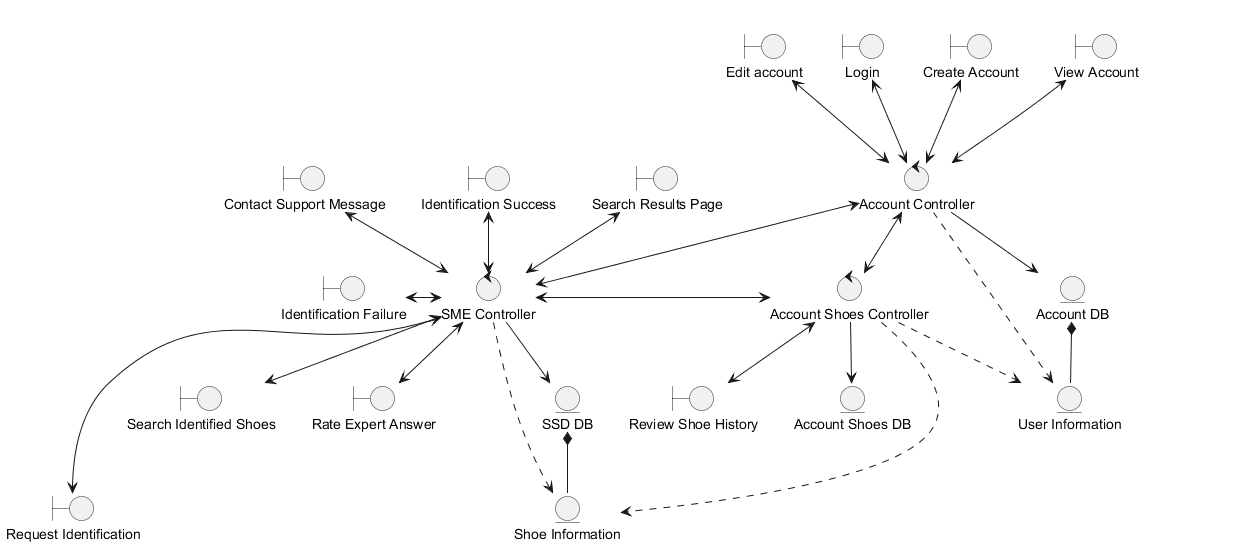
\includegraphics[width = \textwidth]{analysisClassDiagram.png}
	\caption{Analysis Class Diagram}\label{Fig:Q1}
  \end{figure}


% End Section


\section{Architectural Design}
\label{sec:architectural_design}
% Begin Section
This section should provide an overview of the overall architectural design of your application. Your overall architecture should show the division of the system into subsystems with high cohesion and low coupling.

\subsection{System Architecture}
\label{sub:system_architecture}
% Begin SubSection
SoleMate utilizes a Blackboard Architecture integrated with a Repository Style Design to enable efficient shoe identification and data management. The Blackboard Architecture allows multiple expert modules to contribute their analyses iteratively, refining identification results until a final decision is reached. When a user submits a shoe image or textual description, the SoleMate Management Engine (SME Controller) acts as the central hub, posting the input to a shared data space where different expert modules—such as machine learning-based classification, image recognition, and database matching—collaborate to analyze the data. This approach supports a flexible and scalable identification process, allowing for the addition of new expert modules over time and improving recognition accuracy through iterative refinement. \par
The Repository Architecture complements the Blackboard system by ensuring structured and persistent data storage. The SSD Database serves as the repository for storing identified shoes, historical searches, and expert ratings, while the Account Shoes Database and Account Database manage user-related data, such as past searches, stored shoe collections, and authentication details. This repository-style approach allows different subsystems to access data concurrently, ensuring efficient retrieval and updates without conflicts. By combining real-time collaborative processing with structured data management, SoleMate ensures both adaptability and long-term reliability in handling sneaker identification and user interaction. \par
The Blackboard Architecture was chosen because it provides a collaborative problem-solving environment, where different expert modules can iteratively refine identification accuracy. This design is well-suited for SoleMate, as shoe recognition requires integrating various techniques, such as AI models, database lookups, and image recognition. The Repository Architecture was selected to efficiently manage large datasets, ensuring seamless access to stored information while allowing the system to scale as more users and shoe data are added. Together, these architectures provide a flexible, scalable, and data-driven solution for SoleMate’s sneaker identification platform. \par

(Insert diagram here showing SME Controller, SSD Database, expert modules, and subsystem interactions)

Several alternative architectural styles were considered but ultimately discarded. The Model-View-Controller (MVC) Architecture was initially evaluated, but it was not ideal for SoleMate, as the system prioritizes data-driven processing and expert collaboration over UI management. The Pipe and Filter Architecture was also considered but was eliminated because it enforces a sequential flow of data, which does not align with SoleMate’s iterative expert-based approach to identification. Lastly, the Batch Sequential Architecture was rejected due to its reliance on processing data in predefined batches, as SoleMate requires real-time responses for shoe identification requests. By combining Blackboard and Repository Architecture, SoleMate successfully integrates adaptive intelligence with structured data storage, creating an optimal solution for sneaker identification and management.
% End SubSection

\subsection{Subsystems}
\label{sub:subsystems}
% Begin SubSection
% Provide a list of your subsystems, with a brief description of each. Be sure to document its purpose and relationship to other subsystems.

SoleMate utilizes three main subsystems, incorporating both a Blackboard and Repository-like architecture. The SoleMate system integrates a Blackboard Architecture with a repository-style design to streamline shoe identification and user interactions. At the core of the system is the SoleMate Management Engine (SME Controller), which acts as the central coordination unit. When a user submits a shoe identification request through the Request Identification module, the SME Controller processes the request by interacting with different subsystems. The Identification Subsystem plays a key role in this architecture, pulling data from the SSD Database and coordinating with various processing modules to refine identification accuracy. The Account Controller and Account Shoes Controller further support user interactions by managing account-related operations, such as creating, editing, and logging into accounts, as well as storing previously identified shoes for future reference.\par
The repository-style architecture is evident in how SoleMate manages persistent data across various subsystems. The SSD Database functions as the primary data repository, storing shoe identification results, historical searches, and expert ratings. The Account Shoes Database and Account Database store user-specific data, ensuring seamless retrieval of past interactions. The Support and Feedback System allows users to rate expert answers and interact with customer support in case of identification failures. This feedback is stored and utilized by the SME Controller to enhance the system’s future performance. By leveraging a Blackboard approach for expert-driven identification and a repository structure for efficient data storage, SoleMate ensures a robust and scalable platform that enhances user experience and engagement.

% End SubSection

% End Section
	
\section{Class Responsibility Collaboration (CRC) Cards}
\label{sec:class_responsibility_collaboration_crc_cards}
% Begin Section
\begin{table}[H]
    \centering
    \begin{tabular}{|p{0.5\textwidth}|p{0.5\textwidth}|}
        \hline
        \multicolumn{2}{|l|}{\textbf{Class Name:} Account Controller (Controller)} \\
        \hline
        \textbf{Responsibility:} & \textbf{Collaborators:} \\
        \hline
        Knows Edit Account & Edit Account \\
        Knows Login & Login \\
        Knows Create Account  & Create Account\\
        Knows View Account  & View Account \\
        Knows Account DB  & Account DB \\
        Knows User Information  & User Information \\
        Knows Account Shoes Controller & Account Shoes Controller \\
        Knows SME Controller & SME Controller \\
        \hline
    \end{tabular}
    \label{tab:account_controller}
\end{table}

\begin{table}[H]
    \centering
    \begin{tabular}{|p{0.5\textwidth}|p{0.5\textwidth}|}
        \hline
        \multicolumn{2}{|l|}{\textbf{Class Name:} Account Shoes Controller (Controller)} \\
        \hline
        \textbf{Responsibility:} & \textbf{Collaborators:} \\
        \hline
        Knows Account Controller & Account Controller \\
        Knows User Information & User Information \\
        Knows Shoe Information & Shoe Information \\
        Knows Account Shoes DB & Account Shoes DB \\
        Knows Review Shoe History & Review Shoe History \\
        Knows SME Controller & SME Controller \\
        \hline
    \end{tabular}
    \label{tab:account_shoes_controller}
\end{table}

\begin{table}[H]
    \centering
    \begin{tabular}{|p{0.5\textwidth}|p{0.5\textwidth}|}
        \hline
        \multicolumn{2}{|l|}{\textbf{Class Name:} Account DB (Entity)} \\
        \hline
        \textbf{Responsibility:} & \textbf{Collaborators:} \\
        \hline
        Knows Account Controller & Account Controller \\
        Knows User Information & User Information \\
        \hline
    \end{tabular}
    \label{tab:account_db}
\end{table}

\begin{table}[H]
    \centering
    \begin{tabular}{|p{0.5\textwidth}|p{0.5\textwidth}|}
        \hline
        \multicolumn{2}{|l|}{\textbf{Class Name:} Edit Account (Boundary)} \\
        \hline
        \textbf{Responsibility:} & \textbf{Collaborators:} \\
        \hline
        Knows Account Controller & Account Controller \\
        Knows username, password, gender etc. & \\
        Handles click-event of ”Save” button & \\
        \hline
    \end{tabular}
    \label{tab:edit_account}
\end{table}

\begin{table}[H]
    \centering
    \begin{tabular}{|p{0.5\textwidth}|p{0.5\textwidth}|}
        \hline
        \multicolumn{2}{|l|}{\textbf{Class Name:} Login (Boundary)} \\
        \hline
        \textbf{Responsibility:} & \textbf{Collaborators:} \\
        \hline
        Knows Account Controller & Account Controller \\
        Handles click-event of ”login” button &  \\
        \hline
    \end{tabular}
    \label{tab:login}
\end{table}

\begin{table}[H]
    \centering
    \begin{tabular}{|p{0.5\textwidth}|p{0.5\textwidth}|}
        \hline
        \multicolumn{2}{|l|}{\textbf{Class Name:} Create Account (Boundary)} \\
        \hline
        \textbf{Responsibility:} & \textbf{Collaborators:} \\
        \hline
        Knows Account Controller & Account Controller \\
        Knows username and password &  \\
        Handles click-event of ”Create Account” Button & \\
        \hline
    \end{tabular}
    \label{tab:create_account}
\end{table}

\begin{table}[H]
    \centering
    \begin{tabular}{|p{0.5\textwidth}|p{0.5\textwidth}|}
        \hline
        \multicolumn{2}{|l|}{\textbf{Class Name:} View Account (Boundary)} \\
        \hline
        \textbf{Responsibility:} & \textbf{Collaborators:} \\
        \hline
        Knows Account Controller & Account Controller \\
        Handles click-event of ”View Account” button &  \\
        Displays User Information & \\
        \hline
    \end{tabular}
    \label{tab:view_account}
\end{table}

\begin{table}[H]
    \centering
    \begin{tabular}{|p{0.5\textwidth}|p{0.5\textwidth}|}
        \hline
        \multicolumn{2}{|l|}{\textbf{Class Name:} Account Shoes DB (Entity)} \\
        \hline
        \textbf{Responsibilities:} & \textbf{Collaborators:} \\
        \hline
        Knows Account Shoes Controller & Account Shoes Controller \\
        \hline
    \end{tabular}
    \label{tab:account_shoes_db}
\end{table}

\begin{table}[H]
    \centering
    \begin{tabular}{|p{0.5\textwidth}|p{0.5\textwidth}|}
        \hline
        \multicolumn{2}{|l|}{\textbf{Class Name:} User Information (Entity)} \\
        \hline
        \textbf{Responsibilities:} & \textbf{Collaborators:} \\
        \hline
        Knows Account DB & Account DB \\
        Knows Account Controller & Account Controller \\
        Knows Account Shoes Controller & Account Shoes Controller \\
        Knows user information like username, password, gender etc. & \\ 
        
        \hline
    \end{tabular}
    \label{tab:user_information}
\end{table}

\begin{table}[H]
    \centering
    \begin{tabular}{|p{0.5\textwidth}|p{0.5\textwidth}|}
        \hline
        \multicolumn{2}{|l|}{\textbf{Class Name:} Review Shoe History (Boundary)} \\
        \hline
        \textbf{Responsibilities:} & \textbf{Collaborators:} \\
        \hline
        Knows Account Shoes Controller & Account Shoes Controller \\
        \hline
    \end{tabular}
    \label{tab:review_shoe_history}
\end{table}

\begin{table}[H]
    \centering
    \begin{tabular}{|p{0.5\textwidth}|p{0.5\textwidth}|}
        \hline
        \multicolumn{2}{|l|}{\textbf{Class Name:} Rate Expert Answer (Boundary)} \\
        \hline
        \textbf{Responsibilities:} & \textbf{Collaborators:} \\
        \hline
        Knows ratings for expert answers & SME Controller \\
        Handles user input for rating experts' answers  &  \\
        Displays the rating results  &  \\
        \hline
    \end{tabular}
    \label{tab:rate_expert_answer}
\end{table}


\begin{table}[H]
    \centering
    \begin{tabular}{|p{0.5\textwidth}|p{0.5\textwidth}|}
        \hline
        \multicolumn{2}{|l|}{\textbf{Class Name:} Shoe Information (Entity)} \\
        \hline
        \textbf{Responsibilities:} & \textbf{Collaborators:} \\
        \hline
        Knows detailed shoe information & SSD DB \\
        Knows shoe details and features & SME Controller \\
        Handles filtering and search functionalities & Account Shoe Controller \\
        Displays shoe information for users & \\
        \hline
    \end{tabular}
    \label{tab:shoe_information}
\end{table}

\begin{table}[H]
    \centering
    \begin{tabular}{|p{0.5\textwidth}|p{0.5\textwidth}|}
        \hline
        \multicolumn{2}{|l|}{\textbf{Class Name:} Search Identified Shoes (Boundary)} \\
        \hline
        \textbf{Responsibilities:} & \textbf{Collaborators:} \\
        \hline
        Handles shoe identification based on user queries & SME Controller \\
        Displays retrieved and identified shoes &  \\
        Handles sorting options for identified shoes &  \\
        \hline
    \end{tabular}
    \label{tab:search_identified_shoes}
\end{table}


\begin{table}[H]
    \centering
    \begin{tabular}{|p{0.5\textwidth}|p{0.5\textwidth}|}
        \hline
        \multicolumn{2}{|l|}{\textbf{Class Name:} Request Identification (Boundary)} \\
        \hline
        \textbf{Responsibilities:} & \textbf{Collaborators:} \\
        \hline
        Handles requests for shoe identification & SME Controller \\
        Handles initiation of search for shoe identification &  \\
        Knows the status of an identification request  & \\
        \hline
    \end{tabular}
    \label{tab:request_identification}
\end{table}

\begin{table}[h]
    \centering
    \begin{tabular}{|p{0.5\textwidth}|p{0.5\textwidth}|}
        \hline
        \multicolumn{2}{|l|}{\textbf{Class Name:} Search Results Page (Boundary)} \\
        \hline
        \textbf{Responsibilities:} & \textbf{Collaborators:} \\
        \hline
        Displays the results from shoe searches & SME Controller \\
        Displays organized search data to users &  \\
        Handles filtering and sorting of search results &  \\
        Displays links to detailed shoe information &  \\
        \hline
    \end{tabular}
    \label{tab:search_results_page}
\end{table}

\begin{table}[H]
    \centering
    \begin{tabular}{|p{0.5\textwidth}|p{0.5\textwidth}|}
        \hline
        \multicolumn{2}{|l|}{\textbf{Class Name:} SME Controller (Controller)} \\
        \hline
        \textbf{Responsibilities:} & \textbf{Collaborators:} \\
        \hline
        Handles identification outcomes & Identification Success \\  
        Handles system-support communication & Contact Support Message \\  
        Handles user search requests & Search Identified Shoes \\  
        Displays search results & Search Results Page \\  
        Handles user accounts & Account Controller \\  
        Handles user shoe preferences & Account Shoe Controller \\  
        Knows shoe data & Shoe Information \\  
        Handles database access & SSD DB \\  
        Knows expert ratings & Rate Expert Answer \\  
        Handles shoe identification requests & Request Identification \\  
        Displays identification results & Identification Failure\\  
        Displays error messages & \\  
        Handles search filtering and sorting & \\  
        Handles search pagination & \\  
        Knows system-wide data consistency & \\  
        Knows user activity for recommendations & \\  
        \hline
    \end{tabular}
    \label{tab:sme_controller}
\end{table}


\begin{table}[H]
    \centering
    \begin{tabular}{|p{0.5\textwidth}|p{0.5\textwidth}|}
        \hline
        \multicolumn{2}{|l|}{\textbf{Class Name:} Identification Failure (Boundary)} \\
        \hline
        \textbf{Responsibility:} & \textbf{Collaborators:} \\
        \hline
        Handles identification failures & SME Controller \\
        Displays identification failure notification to user & \\
        \hline
    \end{tabular}
    \label{tab:identification_failure}
\end{table}

\begin{table}[H]
    \centering
    \begin{tabular}{|p{0.5\textwidth}|p{0.5\textwidth}|}
        \hline
        \multicolumn{2}{|l|}{\textbf{Class Name:} Identification Success (Boundary)} \\
        \hline
        \textbf{Responsibility:} & \textbf{Collaborators:} \\
        \hline
        Handles successful identification processes & SME Controller \\
        Displays search results after identification & \\
        \hline
    \end{tabular}
    \label{tab:identification_success}
\end{table}

\begin{table}[H]
    \centering
    \begin{tabular}{|p{0.5\textwidth}|p{0.5\textwidth}|}
        \hline
        \multicolumn{2}{|l|}{\textbf{Class Name:} Contact Support Message (Boundary)} \\
        \hline
        \textbf{Responsibility:} & \textbf{Collaborators:} \\
        \hline
        Handles initiating contact with customer support & SME Controller \\
        Displays the support contact information &  \\
        \hline
    \end{tabular}
    \label{tab:contact_support_message}
\end{table}

\begin{table}[H]
    \centering
    \begin{tabular}{|p{0.5\textwidth}|p{0.5\textwidth}|}
        \hline
        \multicolumn{2}{|l|}{\textbf{Class Name:} SSD DB (Entity)} \\
        \hline
        \textbf{Responsibilities:} & \textbf{Collaborators:} \\
        \hline
        Knows shoe-related search results & SME Controller \\
        Displays data for search results & Shoe Information \\
        Knows detailed shoe attributes & \\  
        Knows price trends and availability & \\  
        Handles updates to shoe-related information & \\   
        Handles database indexing and queries & \\  
        \hline
    \end{tabular}
    \label{tab:ssd_db}
\end{table}
% End Section

\appendix
\section{Division of Labour}
\label{sec:division_of_labour}
% Begin Section
Include a Division of Labour sheet which indicates the contributions of each team member. This sheet must be signed by all team members.
% End Section


\end{document}
%------------------------------------------------------------------------------